\chapter{Les différentes technologies}

Au cours de l’histoire plusieurs technologies ont été découvertes afin de fabriquer des condensateurs. Cela nous offre maintenant, un large choix de technologies suivant les utilisations et, ou les valeurs en Farad nécessaires. Afin de mieux comprendre les avantages et les inconvénients de chaque technologie, nous allons en faire une comparaison des plus couramment utilisées. \\ \\

\begin{figure}[!h]
    \centering
    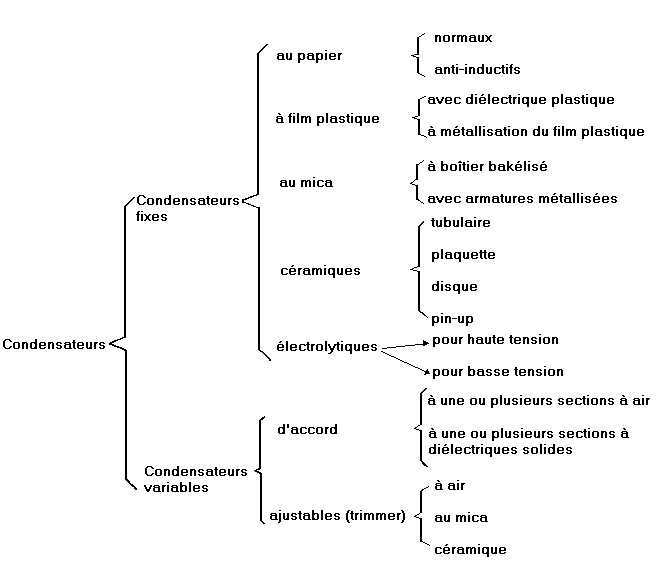
\includegraphics[scale=0.7]{\rootImages/classification.PNG}
    \caption{Classification des différents types de condensateur}
    \label{classification}
\end{figure}

La figure \ref{classification} récapitule tous les types de condensateurs. Ils sont divisés en 2 catégories, les condensateurs à capacité fixes et ceux à capacité variable. Nous allons par la suite nous intéresser majoritairement au condensateur à capacité fixe car ce sont ceux le plus répandus.

\section{Les condensateurs à film}


Ces condensateurs utilisent un film plastique. Il en existe de 2 types, suivant l’utilisation du film plastique.  Ceux de type un utilisent un film plastique comme diélectrique, c’est-à-dire comme moyen de limiter ou empêcher la conduction électrique mais laissant s’exercer les forces électrostatiques. Ceux de type deux utilisent quant à eux un film plastique métallisé. \\


\begin{figure}[!h]
    \centering
    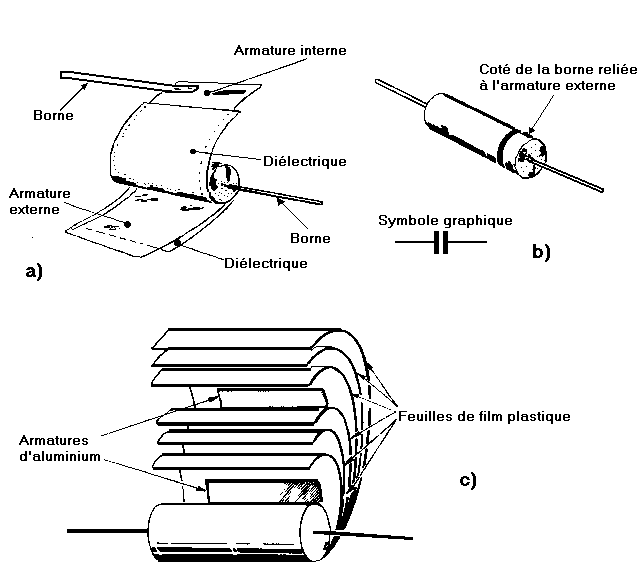
\includegraphics[scale=0.5]{\rootImages/condo_film.png}
    \caption{Schéma interne d'un condensateur à film plastique}
\end{figure}

Ces condensateurs possèdent une faible capacité comprise entre 1nF et 30µF, mais à défaut permettent une très grande précision. Ils possèdent également une durée de vie supérieure à la plupart des autres types de condensateurs et ne sont pas polarisé. De plus, certains de ces condensateurs permettent une régénération après un claquage. Ils sont également conçus pour résister à de hautes tensions (de l’ordre du kilovolt) et permettent de fournir des impulsions de courant de surcharge très élevées.

\newpage
\section{Les condensateurs à céramique}

Ce type de condensateur est celui majoritairement utilisé. Ils sont notamment très utilisés en électronique du fait de leur petite taille. Ils permettent des capacités comprises entre 1nF et 1µF. Ils ne sont pas polarisés comme les condensateurs à film ce qui permet leur utilisation dans des circuits à courant alternatif. Il en existe également 2 types :\\

\begin{itemize}
    \item Ceux de classe 1 sont utilisés lorsque l’on nécessite une grande stabilité et de faible perte. Ils possèdent une valeur de capacité très stable.\\
    \item Ceux de classe 2 possèdent une capacité élevée. Ils perdent cependant en stabilité thermique et les tolérances de capacité sont plus élevée.
\end{itemize}

\begin{figure}[!h]
    \centering
    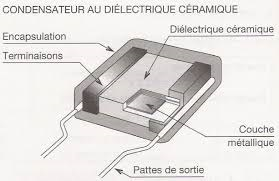
\includegraphics[scale=1]{\rootImages/condo_ceramique.jpg}
    \caption{Schéma interne d'un condensateur à céramique}
\end{figure}


\newpage
\section{Les condensateurs électrolytiques}

Les condensateurs électrolytiques ou encore condensateurs chimiques, utilisent un électrolyte, c’est-à-dire une substance conductrice contenant des ions mobiles. Cela permet à ces condensateurs de pouvoir fournir une plus grande plage de valeur de capacité que les autres types de condensateur. Ils sont dans la très grande majorité polarisé ce qui oblige leur utilisation dans des circuits à courant continu. On en voit très souvent dans des alimentations notamment d'ordinateur etc... Ils permettent une capacité comprise entre 1µF et 47mF avec une tension de fonctionnement pouvant aller à l’ordre de quelques centaines de volts. Ils ne sont cependant pas très précis. En effet il possède une tolérance de 20\%, une grande résistance en série et réagissent très mal aux hautes fréquences (surchauffe). 


\begin{figure}[!h]
    \centering
    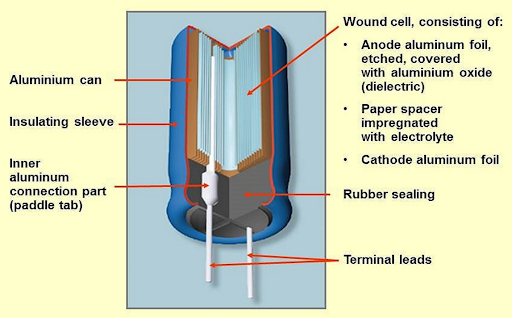
\includegraphics[scale=0.5]{\rootImages/condo_electro.png}
    \caption{Schéma interne d'un condensateur électrolytiques}
\end{figure}


\section{Les condensateurs variables}

Les condensateurs variables sont des condensateurs dont la valeur de la capacité est comme son nom l’indique variable. Ils sont constitués d’un rotor, d’un axe et d’un stator. 

\begin{figure}[!h]
    \centering
    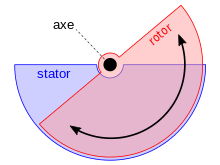
\includegraphics[scale=0.5]{\rootImages/condo_variable.png}
    \caption{Schéma interne d'un condensateur variable}
\end{figure}

Le rotor entraîné par l’axe tourne dans l’armature fixe du stator. La capacité de ces condensateurs varie en continu entre une valeur minimum appelé capacité résiduelle et une valeur maximum appelée capacité nominale. \\

Cette variation suit une fonction appelée loi de variation : 

\begin{align}
    C=f(\theta)
\end{align}

f() dépend de multiples paramètres complexes. Il est donc difficile de pouvoir le définir clairement.\\
$\theta$ quant à lui correspond à l'angle de rotation de l'axe. \\ \\

\begin{figure}[!h]
    \centering
    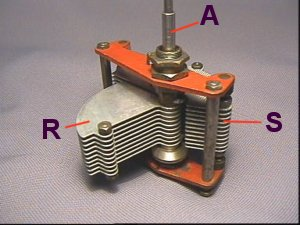
\includegraphics[scale=0.8]{\rootImages/condo_variable.jpg}
    \caption{Condensateur à capacité variable}
\end{figure}


Nous avons pu dans cette partie, nous intéresser à différents types de condensateur. Il en existe encore plein d'autres comme les condensateurs au mica, au papier... Mais nous avons vu ici, ceux les plus couramment utilisés.

